\documentclass[final,xcolor={table}]{beamer}
%% Possible paper sizes: a0, a0b, a1, a2, a3, a4.
%% Possible orientations: portrait, landscape
%% Font sizes can be changed using the scale option.
\usepackage[size=a0,orientation=landscape]{beamerposter}

\usetheme{gemini}
\usecolortheme{seagull}
\useinnertheme{rectangles}
\usefonttheme[onlymath]{serif}


% amsmath
\DeclareMathOperator{\diag}{diag}
\DeclareMathOperator{\tr}{tr}
\DeclareMathOperator{\sv}{sv}
\DeclareMathOperator{\card}{card}
\DeclareMathOperator{\svd}{svd}
\DeclareMathOperator{\rank}{rank}

\setlength\lineskip{20pt}
% \let\OLDitemize\itemize
% \renewcommand\itemize{\OLDitemize\addtolength{\itemsep}{20pt}}
% \renewcommand\baselinestretch{1.25}

% ====================
% Packages
% ====================

% \usepackage[utf8]{inputenc}
% \usepackage[table]{xcolor}
\usepackage{adjustbox}
\usepackage{graphicx}
\usepackage{booktabs}
\usepackage{tikz}
\usepackage{pgfplots}
\usepackage[T1]{fontenc}
\usepackage[sfdefault]{FiraSans}
\usepackage[acronym]{glossaries-extra}
\usepackage{siunitx}
\usepackage[caption=false,font=footnotesize,subrefformat=parens,labelformat=parens]{subfig}
\usepackage{tabularx}
\usepackage{multirow}
\usepackage[american]{circuitikz}
\usepackage[short]{optidef}

\usetikzlibrary{arrows,calc,matrix,patterns,plotmarks,positioning,shapes}
\usetikzlibrary{decorations.pathmorphing,decorations.pathreplacing,decorations.shapes,shapes.geometric}
\usepgfplotslibrary{groupplots,patchplots}
\pgfplotsset{compat=newest}



\glsdisablehyper
\setabbreviationstyle[acronym]{long-short}
\newacronym{ao}{AO}{Alternating Optimization}
\newacronym{bd}{BD}{Beyond Diagonal}
\newacronym{bcd}{BCD}{Block Coordinate Descent}
\newacronym{d}{D}{Diagonal}
\newacronym{dof}{DoF}{Degrees of Freedom}
\newacronym{siso}{SISO}{Single-Input Single-Output}
\newacronym{miso}{MISO}{Multiple-Input Single-Output}
\newacronym{mimo}{MIMO}{Multiple-Input Multiple-Output}
\newacronym{rcg}{RCG}{Riemannian Conjugate Gradient}
\newacronym{ris}{RIS}{Reconfigurable Intelligent Surface}
\newacronym{pc}{PC}{Point-to-point Channel}
\newacronym{ic}{IC}{Interference Channel}
\newacronym{wsr}{WSR}{Weighted Sum-Rate}
\newacronym{snr}{SNR}{Signal-to-Noise Ratio}
\newacronym{svd}{SVD}{Singular Value Decomposition}
\newacronym{mmse}{MMSE}{Minimum Mean-Square Error}
\newacronym{wmmse}{WMMSE}{Weighted \gls{mmse}}
\newacronym{mse}{MSE}{Mean-Square Error}
\newacronym{los}{LoS}{Line-of-Sight}
\newacronym{csi}{CSI}{Channel State Information}
\newacronym{cscg}{CSCG}{Circularly Symmetric Complex Gaussian}
\newacronym{sca}{SCA}{Successive Convex Approximation}
\newacronym{kkt}{KKT}{Karush-Kuhn-Tucker}



% ====================
% Lengths
% ====================

% If you have N columns, choose \sepwidth and \colwidth such that
% (N+1)*\sepwidth + N*\colwidth = \paperwidth
\newlength{\sepwidth}
\newlength{\colwidth}
\setlength{\sepwidth}{0.025\paperwidth}
\setlength{\colwidth}{0.3\paperwidth}
% \setlength{\sepwidth}{0.03\paperwidth}
% \setlength{\colwidth}{0.45\paperwidth}

\newcommand{\separatorcolumn}{\begin{column}{\sepwidth}\end{column}}

% ====================
% Logo (optional)
% ====================

% LaTeX logo taken from https://commons.wikimedia.org/wiki/File:LaTeX_logo.svg
% use this to include logos on the left and/or right side of the header:
\logoleft{\includegraphics[height=1.5cm]{../assets/poster/logo_imperial.eps}}
\logoright{\includegraphics[height=4cm]{../assets/poster/qrcode_github.png}}

% ====================
% Footer (optional)
% ====================

\footercontent{
	IEEE ComSoc Workshops @ ICL \hfill
	November 25 \& 26, 2024 \hfill
	\href{mailto:yang.zhao@ieee.org}{yang.zhao@ieee.org}
}
% (can be left out to remove footer)

% ====================
% My own customization
% - BibLaTeX
% - Boxes with tcolorbox
% - User-defined commands
% ====================
\input{custom-defs.tex}

%% Reference Sources
% \addbibresource{library.bib}
\renewcommand{\pgfuseimage}[1]{\includegraphics[scale=2.0]{#1}}

\title{Channel Shaping Using Beyond Diagonal RIS: Analysis, Optimization, and Enhanced Flexibility}

\author{Yang Zhao \and Hongyu Li \and Massimo Franceschetti \and Bruno Clerckx}

\date{January 01, 2025}

\begin{document}

\begin{frame}[t]
	\begin{columns}[t]
		\separatorcolumn

		\begin{column}{\colwidth}
			\begin{block}{Overview}
				\begin{itemize}\setlength\itemsep{20pt}
					\item \textbf{What does this paper investigate?}

					The capability of \gls{d} and \gls{bd} \gls{ris} to redistribute the singular values of \glsfmtshort{mimo} channels.
					\item \textbf{How does it differ from previous work?}

					It derives analytical singular value bounds for specific channel conditions. And proposes a novel \gls{bd}-\gls{ris} optimization framework for general problems.
					\item \textbf{What are the benefits?}

					\gls{bd}-\gls{ris} improves the dynamic range of individual channel singular values and the trade-off in manipulating them. This boosts channel power gain and capacity.
				\end{itemize}
			\end{block}

			\begin{block}{\gls{bd}-\gls{ris} model}
				\setlength{\leftskip}{\leftmargini}
				\setlength{\rightskip}{\leftmargini}
				Consider an $N_\mathrm{T} \times N_\mathrm{S} \times N_\mathrm{R}$ setup with \gls{bd}-\gls{ris} divided into $G$ groups of $L$ elements each.
				Define $N = \min(N_\mathrm{T}, N_\mathrm{R})$, $\bar{N} = \max(N_\mathrm{T}, N_\mathrm{S}, N_\mathrm{R})$, and $\mathbf{H}_{\mathrm{B}/\mathrm{F}}\stackrel{\svd}{=} \mathbf{U}_{\mathrm{B}/\mathrm{F}} \boldsymbol{\Sigma}_{\mathrm{B}/\mathrm{F}} \mathbf{V}_{\mathrm{B}/\mathrm{F}}^\mathsf{H}$.
				\begin{equation*}
					\mathbf{\Theta} = \diag(\mathbf{\Theta}_1,\ldots,\mathbf{\Theta}_G),\quad \mathbf{\Theta}_g^\mathsf{H} \mathbf{\Theta}_g = \mathbf{I}_L \ \forall g, \quad \mathbf{H} = \overbrace{\mathbf{H}_\mathrm{D} + \sum\nolimits_g \underbrace{\mathbf{H}_{\mathrm{B},g} \mathbf{\Theta}_g \mathbf{H}_{\mathrm{F},g}}_{\small{\substack{\text{backward-forward:}\\\text{intra-group, multiplicative}}}}}^{\small{\substack{\text{direct-indirect:}\\\text{inter-group, additive}}}}.
				\end{equation*}

				\begin{itemize}
					\setlength{\rightskip}{\leftmargini}
					\item \textcolor{imperialblue}{Branch matching:} Pairing and combining the entries of $\mathbf{H}_{\mathrm{B},g}$ and $\mathbf{H}_{\mathrm{F},g}$ through unitary transformation $\mathbf{\Theta}_g$.
					\item \textcolor{imperialblue}{Mode alignment:} Aligning and ordering the singular vectors of $\{\mathbf{H}_g\}$ with those of $\mathbf{H}_\mathrm{D}$ through unitary transformations $\{\mathbf{\Theta}_g\}$.
				\end{itemize}
			\end{block}

			\begin{exampleblock}{Example 1: \glsfmtshort{siso} channel gain maximization}
				\setlength{\leftskip}{\leftmargini}
				\setlength{\rightskip}{\leftmargini}
				\glsfmtshort{siso} mode alignment reduces to phase matching and any $L$ (incl. \gls{d}-\gls{ris}) suffices by
				\begin{equation*}
					\mathbf{\Theta}_g^\text{\gls{siso}} = \frac{h_\mathrm{D}}{\lvert h_\mathrm{D} \rvert} \mathbf{V}_{\mathrm{B},g} \mathbf{U}_{\mathrm{F},g}^\mathsf{H} \ \forall g,
					\label{eq:scattering_siso}
				\end{equation*}
				where $\mathbf{V}_{\mathrm{B},g} = \bigl[\mathbf{h}_{\mathrm{B},g}/\lVert \mathbf{h}_{\mathrm{B},g} \rVert, \mathbf{N}_{\mathrm{B},g}\bigr]$, $\mathbf{U}_{\mathrm{F},g} = \bigl[\mathbf{h}_{\mathrm{F},g}/\lVert \mathbf{h}_{\mathrm{F},g} \rVert, \mathbf{N}_{\mathrm{F},g}\bigr]$, and $\mathbf{N}_{\mathrm{B},g}, \mathbf{N}_{\mathrm{F},g}$ are orthonormal bases of null spaces of $\mathbf{h}_{\mathrm{B},g}, \mathbf{h}_{\mathrm{F},g}$.
				The channel gain is a function of $L$
				\begin{equation*}
					\max\nolimits_{\mathbf{\Theta}_{\mathrm{BD}}} \ \lvert h \rvert = \lvert h_\mathrm{D} \rvert + \sum\nolimits_g \sum\nolimits_l \lvert h_{\mathrm{B},g,\pi_{\mathrm{B},g}(l)} \rvert \lvert h_{\mathrm{F},g,\pi_{\mathrm{F},g}(l)} \rvert,
				\end{equation*}
				which generalizes $\max_{\mathbf{\Theta}_{\mathrm{D}}} \ \lvert h \rvert = \lvert h_\mathrm{D} \rvert + \sum_{n=1}^{N_\mathrm{S}} \lvert h_{\mathrm{B},n} \rvert \lvert h_{\mathrm{F},n} \rvert$ using permutations $\pi_{\mathrm{B},g}, \pi_{\mathrm{F},g}$ that pair the $l$-th strongest backward and forward branches.
				% This generalizes $\max_{\mathbf{\Theta}_{\mathrm{D}}} \ \lvert h \rvert = \lvert h_\mathrm{D} \rvert + \sum_{n=1}^{N_\mathrm{S}} \lvert h_{\mathrm{B},n} \rvert \lvert h_{\mathrm{F},n} \rvert$.
			\end{exampleblock}


			\begin{exampleblock}{Example 2: $2 \times 2 \times 2$ shaping}
				\setlength{\leftskip}{\leftmargini}
				\setlength{\rightskip}{\leftmargini}
				\gls{d}-\gls{ris} and fully-connected \gls{bd}-\gls{ris} can be modeled by 2 and 4 angular parameters:
				\begin{equation*}
					\mathbf{\Theta}_\mathrm{D} = \diag(e^{\jmath \theta_1}, e^{\jmath \theta_2}), \quad
					\mathbf{\Theta}_\mathrm{BD} = e^{\jmath \phi} \begin{bmatrix}
						e^{\jmath \alpha} \cos \psi  & e^{\jmath \beta} \sin \psi   \\
						-e^{-\jmath \beta} \sin \psi & e^{-\jmath \alpha} \cos \psi
					\end{bmatrix}.
				\end{equation*}

				Assume the \gls{bd}-\gls{ris} is symmetric (i.e., $\beta = \pi / 2$) and the direct channel is negligible (i.e., $\sv(e^{\jmath \phi} \mathbf{A}) = \sv(\mathbf{A})$).
				The plot relies on grid search for one channel realization.
				\begin{figure}
					\centering
					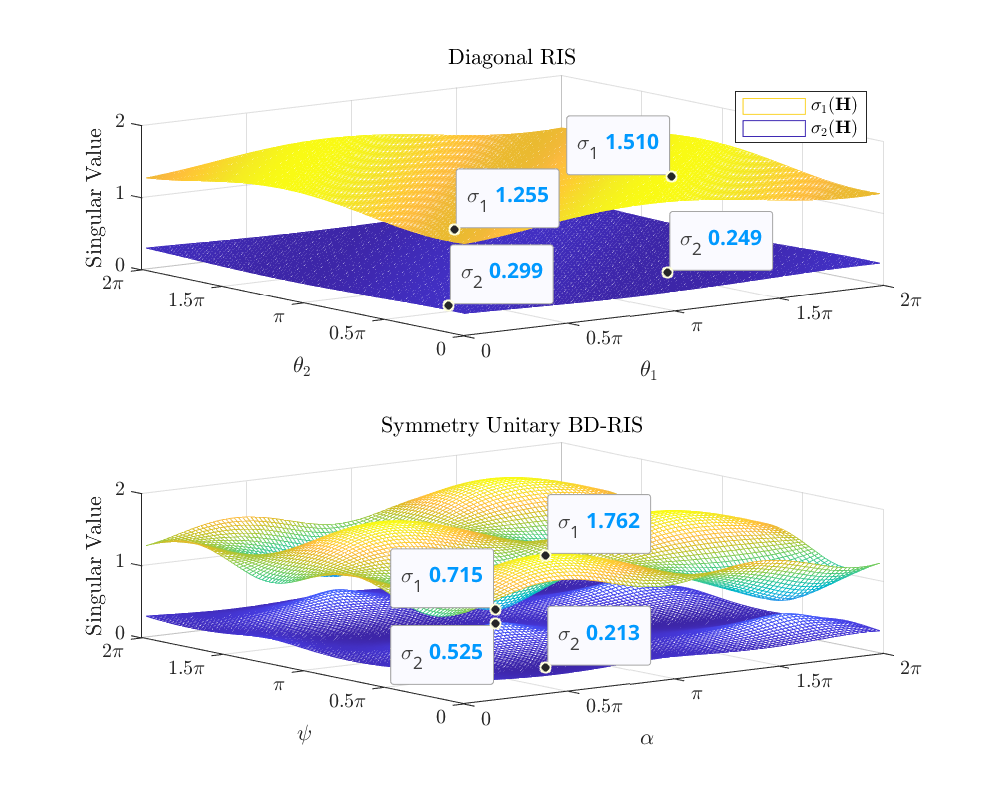
\includegraphics[width=0.44\columnwidth]{../assets/simulation/singular_trend.eps}
					% \caption{
					% 	\setlength{\leftskip}{\leftmargini}
					% 	\setlength{\rightskip}{\leftmargini}
					% 	Singular value shaping by \gls{d}-\gls{ris} and symmetric fully-connected \gls{bd}-\gls{ris}.
					% 	The maximum and minimum singular values are marked explicitly on the plot.}
				\end{figure}
				Here, both singular values are manipulated up to $\pm 9\%$ by \gls{d}-\gls{ris} and $\pm 42\%$ by symmetric fully-connected \gls{bd}-\gls{ris}, using 2 and 3 circuit components respectively.
			\end{exampleblock}
		\end{column}

		\separatorcolumn

		\begin{column}{\colwidth}
			\vspace{-0.5cm}
			\begin{prop}{\gls{dof}}{}
				\setlength{\leftskip}{\leftmargini}
				\setlength{\rightskip}{\leftmargini}
				In point-to-point \glsfmtshort{mimo}, \gls{bd}-\gls{ris} cannot achieve a larger number of \gls{dof} than \gls{d}-\gls{ris}.
			\end{prop}

			\begin{prop}{Rank-deficient channels}{}
				\setlength{\leftskip}{\leftmargini}
				\setlength{\rightskip}{\leftmargini}
				If the minimum rank of backward and forward channels is $k$,
				then for \gls{d}-\gls{ris} or \gls{bd}-\gls{ris} of arbitrary number of elements, the $n$-th channel singular value is bounded by
				\begin{align*}
					\sigma_n(\mathbf{H}) & \le \sigma_{n-k}(\mathbf{T}), &  & \text{if } n > k, \\
					\sigma_n(\mathbf{H}) & \ge \sigma_n(\mathbf{T}),     &  & \text{if } n < N - k + 1,
				\end{align*}
				where $\mathbf{T}$ is arbitrary auxiliary matrix satisfying
				\begin{equation*}
					\mathbf{T} \mathbf{T}^\mathsf{H} =
					\begin{cases}
						\mathbf{H}_\mathrm{D} (\mathbf{I} - \mathbf{V}_\mathrm{F} \mathbf{V}_\mathrm{F}^\mathsf{H}) \mathbf{H}_\mathrm{D}^\mathsf{H}, & \text{if } \mathrm{rank}(\mathbf{H}_\mathrm{F}) = k, \\
						\mathbf{H}_\mathrm{D}^\mathsf{H} (\mathbf{I} - \mathbf{U}_\mathrm{B} \mathbf{U}_\mathrm{B}^\mathsf{H}) \mathbf{H}_\mathrm{D}, & \text{if } \mathrm{rank}(\mathbf{H}_\mathrm{B}) = k.
					\end{cases}
				\end{equation*}
				\vspace{-0.5cm}
			\end{prop}

			\begin{coro}{\gls{los} channel}{}
				\setlength{\leftskip}{\leftmargini}
				\setlength{\rightskip}{\leftmargini}
				If one of backward and forward channels is \gls{los}, then a \gls{d}-\gls{ris} or \gls{bd}-\gls{ris} can only manipulate the channel singular values up to
				\begin{equation*}
					\sigma_1(\mathbf{H}) \ge \sigma_1(\mathbf{T}) \ge {\sigma_2(\mathbf{H})} \ge \ldots \ge \sigma_{N-1}(\mathbf{T}) \ge {\sigma_N(\mathbf{H})} \ge \sigma_N(\mathbf{T}).
				\end{equation*}
				As $N_\mathrm{S} \to \infty$, $N$ out of those $2N$ bounds can be \emph{simultaneously} tight.
			\end{coro}

			\begin{prop}{Negligible direct channel}{}
				\setlength{\leftskip}{\leftmargini}
				\setlength{\rightskip}{\leftmargini}
				If the direct channel is negligible, then a fully-connected \gls{bd}-\gls{ris} can manipulate the channel singular values up to
				\begin{equation*}
					\sv(\mathbf{H}) = \sv(\mathbf{BF}),
				\end{equation*}
				where $\mathbf{B}$ and $\mathbf{F}$ are arbitrary matrices with $\sv(\mathbf{B})=\sv(\mathbf{H}_\mathrm{B})$ and $\sv(\mathbf{F})=\sv(\mathbf{H}_\mathrm{F})$.
			\end{prop}

			\setcounter{coro}{2}

			\begin{coro}{Individual singular value}{}
				\setlength{\leftskip}{\leftmargini}
				\setlength{\rightskip}{\leftmargini}
				If the direct channel is negligible,
				then the $n$-th channel singular value is bounded by
				\begin{equation*}
					\max_{i+j=n+N_\mathrm{S}} \sigma_i(\mathbf{H}_\mathrm{B}) \sigma_j(\mathbf{H}_\mathrm{F}) \le \sigma_n(\mathbf{H}) \le \min_{i+j=n+1} \sigma_i(\mathbf{H}_\mathrm{B}) \sigma_j(\mathbf{H}_\mathrm{F}),
				\end{equation*}
				which are attained respectively at
				\begin{equation*}
					\mathbf{\Theta}_{\text{sv-}n\text{-max}}^\text{MIMO-ND} = \mathbf{V}_\mathrm{B} \mathbf{P} \mathbf{U}_\mathrm{F}^\mathsf{H}, \quad \mathbf{\Theta}_{\text{sv-}n\text{-min}}^\text{MIMO-ND} = \mathbf{V}_\mathrm{B} \mathbf{Q} \mathbf{U}_\mathrm{F}^\mathsf{H},
				\end{equation*}
				where $\mathbf{P}, \mathbf{Q}$ are permutation matrices of dimension $N_\mathrm{S}$ satisfying:
				\begin{itemize}\color{black}
					\item The $(i, j)$-th entry is $1$, where
					\begin{equation*}
						(i, j) =
						\begin{cases}
							\underset{i+j=n+1}{\arg\min} \sigma_i(\mathbf{H}_\mathrm{B}) \sigma_j(\mathbf{H}_\mathrm{F}) & \text{ for } \mathbf{P}, \\
							\underset{i+j=n+N_\mathrm{S}}{\arg\max} \sigma_i(\mathbf{H}_\mathrm{B}) \sigma_j(\mathbf{H}_\mathrm{F}) & \text{ for } \mathbf{Q},
						\end{cases}
					\end{equation*}
					and ties may be broken arbitrarily;
					\item After deleting the $i$-th row and $j$-th column, the resulting submatrix $\mathbf{Y}$ is arbitrary permutation matrix of dimension $N_\mathrm{S}-1$ satisfying
					\begin{alignat*}{2}
						\sigma_{n{-}1}(\hat{\mathbf{\Sigma}}_{\mathrm{B}} \mathbf{Y} \hat{\mathbf{\Sigma}}_{\mathrm{F}}) & {\ge} \min_{i+j=n+1} \sigma_i(\mathbf{H}_\mathrm{B}) \sigma_j(\mathbf{H}_\mathrm{F}) && \text{ for } \mathbf{P}, \\
						\sigma_{n{+}1}(\hat{\mathbf{\Sigma}}_{\mathrm{B}} \mathbf{Y} \hat{\mathbf{\Sigma}}_{\mathrm{F}}) & {\le} \max_{i+j=n+N_\mathrm{S}} \sigma_i(\mathbf{H}_\mathrm{B}) \sigma_j(\mathbf{H}_\mathrm{F}) && \text{ for } \mathbf{Q},
					\end{alignat*}
					where $\hat{\mathbf{\Sigma}}_{\mathrm{B}}, \hat{\mathbf{\Sigma}}_{\mathrm{F}}$ are ${\mathbf{\Sigma}}_{\mathrm{B}}, {\mathbf{\Sigma}}_{\mathrm{F}}$ with both $i$-th row and $j$-th column deleted.
				\end{itemize}
			\end{coro}

			\begin{coro}{Channel power gain}{}
				\setlength{\leftskip}{\leftmargini}
				\setlength{\rightskip}{\leftmargini}
				If the direct channel is negligible, then the channel power gain is bounded by
				\begin{equation*}
					\sum\nolimits_{n=1}^N \sigma_n^2(\mathbf{H}_\mathrm{B}) \sigma_{N_\mathrm{S}-n+1}^2(\mathbf{H}_\mathrm{F}) \le \lVert \mathbf{H} \rVert _\mathrm{F}^2 \le \sum\nolimits_{n=1}^N \sigma_n^2(\mathbf{H}_\mathrm{B}) \sigma_n^2(\mathbf{H}_\mathrm{F}),
				\end{equation*}
				which are attained respectively at
				\begin{equation*}
					\mathbf{\Theta}_\text{P-max}^\text{MIMO-ND} = \mathbf{V}_\mathrm{B} \mathbf{U}_\mathrm{F}^\mathsf{H}, \quad \mathbf{\Theta}_\text{P-min}^\text{MIMO-ND} = \mathbf{V}_\mathrm{B} \mathbf{J} \mathbf{U}_\mathrm{F}^\mathsf{H},
				\end{equation*}
				where $\mathbf{J}$ is the backward identity matrix.
			\end{coro}

			\begin{coro}{Channel capacity at very low and high \glsfmtshort{snr}}{}
				\setlength{\leftskip}{\leftmargini}
				\setlength{\rightskip}{\leftmargini}
				If the direct channel is negligible, then the channel capacity at very low and high \glsfmtshort{snr} are approximately bounded from above by
				\begin{align*}
					C_{\rho_\downarrow} & \lessapprox \sigma_1^2(\mathbf{H}_\mathrm{B}) \sigma_1^2(\mathbf{H}_\mathrm{F}), \\
					C_{\rho_\uparrow} & \lessapprox N \log \frac{\rho}{N} + 2 \log \prod\nolimits_{n=1}^N \sigma_n(\mathbf{H}_\mathrm{B}) \sigma_n(\mathbf{H}_\mathrm{F}).
				\end{align*}
				Their upper bounds can be attained at, for example, $\mathbf{\Theta}_\text{P-max}^\text{MIMO-ND}$.
			\end{coro}
		\end{column}

		\separatorcolumn

		\begin{column}{\colwidth}
			\vspace{-0.5cm}
			\begin{algo}{Group-wise geodesic optimization}{}
				\setlength{\leftskip}{\leftmargini}
				\setlength{\rightskip}{\leftmargini}
				% A geodesic is a curve representing the shortest path between two points in a Riemannian manifold.
				For \gls{bd}-\gls{ris} optimization problem of the form
				\begin{maxi*}
					{\scriptstyle{\mathbf{\Theta}}}{f(\mathbf{\Theta})}{}{}
					\addConstraint{\mathbf{\Theta}_g^\mathsf{H} \mathbf{\Theta}_g=\mathbf{I},}{\quad \forall g,}{}
				\end{maxi*}
				% At iteration $r$, the $g$-th group is updated by \textcolor{imperialblue}{geodesic} \gls{rcg}
				we propose a \textcolor{pink!50!pink!75!black}{geodesic} \gls{rcg} algorithm below.
				\vspace{0.5cm}

				\begin{enumerate}\color{black}
					\item \emph{Compute the Euclidean gradient:}
					\begin{equation*}
						\nabla_{\mathrm{E},g}^{(r)} = \frac{\partial f(\mathbf{\Theta}_g^{(r)})}{\partial \mathbf{\Theta}_g^*};
					\end{equation*}
					\item \emph{Translate to the Riemannian gradient evaluated at the identity:}
					\begin{equation*}
						\tilde{\nabla}_{\mathrm{R},g}^{(r)} = \nabla_{\mathrm{E},g}^{(r)} \mathbf{\Theta}_g^{(r)\mathsf{H}} - \mathbf{\Theta}_g^{(r)} {\nabla_{\mathrm{E},g}^{(r)\mathsf{H}}};
					\end{equation*}
					\item \emph{Determine the conjugate direction:}
					\begin{equation*}
						{\mathbf{D}}_g^{(r)} = \tilde{\nabla}_{\mathrm{R},g}^{(r)} + \tilde{\gamma}_g^{(r)} {\mathbf{D}}_g^{(r-1)}, \quad \tilde{\gamma}_g^{(r)} = \frac{\tr\bigl((\tilde{\nabla}_{\mathrm{R},g}^{(r)} - \tilde{\nabla}_{\mathrm{R},g}^{(r-1)}) {\tilde{\nabla}_{\mathrm{R},g}^{(r)\mathsf{H}}}\bigr)}{\tr\bigl(\tilde{\nabla}_{\mathrm{R},g}^{(r-1)} {\tilde{\nabla}_{\mathrm{R},g}^{(r-1)\mathsf{H}}}\bigr)};
					\end{equation*}
					\item \emph{Perform \textcolor{pink!50!pink!75!black}{multiplicative} update along geodesic:}
					\begin{equation*}
						\mathbf{\Theta}_g^{(r+1)} = \mathbf{G}_g^{(r)}(\mu) = \exp(\mu \mathbf{D}_g^{(r)}) \mathbf{\Theta}_g^{(r)},
					\end{equation*}
					where $\mu$ is refinable by the Armijo rule.
				\end{enumerate}
				\vspace{0.5cm}
			\end{algo}

			\begin{exampleblock}{Result 1: Algorithm evaluation}
				\begin{table}[!t]
					\centering
					\begin{tabular}{ccccccc}
						\toprule
						\multirow{2}{*}{\gls{rcg} path} & \multicolumn{3}{c}{$N_\mathrm{S}=16$} & \multicolumn{3}{c}{$N_\mathrm{S}=256$}                                                                     \\ \cmidrule(lr){2-4} \cmidrule(lr){5-7}
														& Objective                             & Iterations                               & Time [s]         & Objective        & Iterations   & Time [s]   \\ \midrule
						Geodesic                        & $\num{4.359e-3}$                      & $11.59$                                  & $\num{1.839e-2}$ & $\num{1.163e-2}$ & $25.58$      & $3.461$    \\
						Non-geodesic                    & $\num{4.329e-3}$                      & $30.92$                                  & $\num{5.743e-2}$ & $\num{1.116e-2}$ & $61.40$      & $13.50$    \\ \bottomrule
					\end{tabular}
				\end{table}
			\end{exampleblock}

			\begin{exampleblock}{Result 2: Bounds and Pareto frontier of singular values}
				\begin{figure}[!t]
					\centering
					\subfloat[Analytical vs numerical results: $4 \times 128 \times 4, \rank(\mathbf{H}_\mathrm{F}) = 2$]{
						\resizebox{0.492\linewidth}{!}{
							\input{../assets/poster/singular_bound_rank2_sx128.tex}
						}
					}
					\subfloat[Pareto frontier: $2 \times 64 \times 2$]{
						\resizebox{0.462\linewidth}{!}{
							% This file was created by matlab2tikz.
%
%The latest updates can be retrieved from
%  http://www.mathworks.com/matlabcentral/fileexchange/22022-matlab2tikz-matlab2tikz
%where you can also make suggestions and rate matlab2tikz.
%
\definecolor{mycolor1}{rgb}{0.00000,0.44706,0.74118}%
\definecolor{mycolor2}{rgb}{0.85098,0.32549,0.09804}%
\definecolor{mycolor3}{rgb}{0.92941,0.69412,0.12549}%
\definecolor{mycolor4}{rgb}{0.49412,0.18431,0.55686}%
%
\begin{tikzpicture}

\begin{axis}[%
	width=9.509cm,
	height=7.5cm,
at={(0cm,0cm)},
scale only axis,
xmin=0.000665933747270548,
xmax=0.00180816416675568,
% xlabel style={font=\color{white!15!black}},
xlabel={$\sigma_1(\mathbf{H})$},
ymin=1.10708260774394e-20,
ymax=0.000931271909489233,
% ylabel style={font=\color{white!15!black}},
ylabel={$\sigma_2(\mathbf{H})$},
axis background/.style={fill=white},
xmajorgrids,
ymajorgrids,
legend style={at={(0.03,0.03)}, anchor=south west, legend cell align=left, align=left, draw=white!15!black},
every axis plot/.append style={line width=1.5pt},
x tick scale label style={yshift=7pt},
x label style={yshift=10pt},
y label style={yshift=-7pt}
]
\addplot[only marks, mark=triangle, mark options={}, mark size=2.3570pt, draw=black] table[row sep=crcr]{%
x	y\\
0.00123451554249979	0.000261671419241521\\
};
\addlegendentry{Direct}

\addplot [color=mycolor1, line width=2.0pt, mark=o, mark options={solid, mycolor1}]
  table[row sep=crcr]{%
0.00159608285697502	0.000664114392083429\\
0.00158691664294714	0.000672837941128764\\
0.00157660050010728	0.000681731690268777\\
0.00156590259762528	0.000690085825238813\\
0.00155467994239563	0.000697976645701225\\
0.00153986973643909	0.000707372645028292\\
0.0015148645023757	0.000721449433364078\\
0.00149697676532785	0.000730394195338623\\
0.0014811063630021	0.000737471285391353\\
0.00146705261153674	0.000742888836825103\\
0.00145145312317651	0.000748034879132762\\
0.00143354032724506	0.000752981116885134\\
0.00141219815168891	0.00075775662502572\\
0.00138599656893751	0.000762282978521517\\
0.001355981991655	0.00076597328234428\\
0.00132155867810352	0.000768494850647513\\
0.00127159845792326	0.000769595351798804\\
0.00123642786506839	0.000768807421978087\\
0.00121422536014095	0.000767187754726459\\
0.00118743020096022	0.000763797105859703\\
0.00116236115681128	0.000759517337937116\\
0.00114216255507682	0.000754981192412643\\
0.00112132876332356	0.000749208839458789\\
0.0010987179355452	0.000741727590503771\\
0.001073267755154	0.000731896088791152\\
0.00104840588147425	0.00072089161304077\\
0.00103123882758884	0.000712332026035008\\
0.00102072542642717	0.00070661151546976\\
0.00101127064407598	0.000700865695981975\\
0.00100290573808909	0.000695274516366674\\
0.00099405869556404	0.000688750411001148\\
0.000985723184951612	0.000681989259163176\\
0.000977942269806648	0.000675005939163037\\
0.000883365237789003	0.000578594721583551\\
0.000875259823033198	0.000568804316998415\\
0.00086636420891398	0.000556929660283238\\
0.000858029700529914	0.000544803768004766\\
0.000849145080144272	0.00053057937604649\\
0.000840385049788102	0.00051511967478722\\
0.000831240490517266	0.000497160206301654\\
0.000823405081875965	0.000479893545133291\\
0.000814633564461672	0.000458113314889421\\
0.000806977608550476	0.000436163726292382\\
0.000800072243550595	0.000412970991852368\\
0.000793559072159092	0.000386530995276439\\
0.000788411273090975	0.000360210129693543\\
0.000784467319171457	0.000332879132259079\\
0.000781370109809877	0.000300494465576911\\
0.000779229604973693	0.000255973167522945\\
0.000778843765690314	0.000189061764117299\\
0.000780851644081482	0.00014653579410713\\
0.00078386863842555	0.000116085317999348\\
0.000787435958310619	9.41678760729649e-05\\
0.00079298844062422	6.9432611338902e-05\\
0.000797722113984264	5.34238131636791e-05\\
0.000802073424201546	4.09329153574363e-05\\
0.000806203726326662	3.06917584825308e-05\\
0.000813014934977753	2.20160208093019e-05\\
0.000824950988932121	7.10447651041556e-06\\
0.000827696888811626	3.85134078631187e-06\\
0.000830547864235395	1.21674953920938e-06\\
0.000831965275229041	2.44617826405831e-07\\
0.000832649165431366	1.79133867425279e-08\\
0.000832828850348146	1.10708260774394e-20\\
0.00161378237741308	6.65749607101577e-19\\
0.00161378237741355	5.8393880144134e-16\\
0.00161378237849435	1.32872382628457e-12\\
0.00161639227547958	3.40455067607412e-06\\
0.00163014580907626	2.28971513147335e-05\\
0.00163990293192521	3.82518884070967e-05\\
0.00164673659382605	5.02988168914937e-05\\
0.00165256368270938	6.18735109090836e-05\\
0.00165770600095059	7.34703347459089e-05\\
0.00166401148822954	8.99928952340316e-05\\
0.00167059283856931	0.000109936635373391\\
0.00167658908453108	0.00013162628400113\\
0.00168183527674099	0.000155018775367617\\
0.00168631721115301	0.000180982050508911\\
0.00169157776515169	0.000222197499567037\\
0.0016938416476388	0.000253372151620205\\
0.00169524815187732	0.000327486553761353\\
0.00169398163691352	0.000384104665758756\\
0.00169113344593976	0.000423595412164682\\
0.00168746779562959	0.00045341619951097\\
0.00168166868784352	0.000486331065994069\\
0.00167573939279825	0.000513052824819554\\
0.00166982471571825	0.000534440995798568\\
0.00166328466709128	0.000554261223027059\\
0.00165659661416354	0.000571625272087831\\
0.00164994826526868	0.00058664202350194\\
0.00164324082244803	0.000599976257139259\\
0.00163623992074054	0.000612337398149498\\
0.00162880459408019	0.00062408033199365\\
0.00162098454625344	0.000635186241435433\\
0.00161290650953524	0.00064554019696715\\
0.00160463337370114	0.000655133158519538\\
0.00159608285697502	0.000664114392083429\\
};
\addlegendentry{$L = 1$}

\addplot [color=mycolor2, dashed, line width=2.0pt, mark=+, mark options={solid, mycolor2}]
  table[row sep=crcr]{%
0.0017386594129955	0.000860048272090083\\
0.00173620516066716	0.000862385276306713\\
0.00173365845469748	0.000864582194303698\\
0.00173100324095088	0.000866654293858911\\
0.00172822270935142	0.000868612367139377\\
0.00172529641442896	0.000870465091689542\\
0.00172219949784328	0.000872218997274339\\
0.00171890327802487	0.000873877536139426\\
0.00171537346710331	0.000875441416860692\\
0.00171156313466259	0.00087691025673575\\
0.00170742153093652	0.000878277201093898\\
0.00170288236322903	0.00087953179778277\\
0.00169786056348726	0.000880657548119832\\
0.00169224883215724	0.000881628811261486\\
0.00168591886705108	0.000882406429632005\\
0.00167869706302702	0.000882935175885586\\
0.00167037980039834	0.000883134115394112\\
0.00102052209736536	0.000882801692620656\\
0.00101646047276367	0.000882503284497043\\
0.00101267238345347	0.000882037044403964\\
0.00100912045073618	0.000881421520159389\\
0.00100577415829649	0.000880670753564986\\
0.00100260461810987	0.000879794177847139\\
0.000999591303638097	0.00087879914985014\\
0.000996714501147741	0.000877689800195453\\
0.000993956695076467	0.000876467622492497\\
0.000991304163226718	0.000875132632656254\\
0.00098874401757588	0.000873682418028017\\
0.00098626581874889	0.000872113116072078\\
0.000983859443434805	0.000870418263617197\\
0.000982667940276653	0.000869508063587063\\
0.000980791270287472	0.00086797495643917\\
0.000978764853396329	0.000866174303123083\\
0.00073858103322915	0.000625587747554838\\
0.000736804562629995	0.00062341605253277\\
0.000735216509742291	0.000621195965101899\\
0.000733326042401016	0.000618190330161238\\
0.000731462763390808	0.000614635580866718\\
0.00072960197688474	0.000610261186413097\\
0.000727481471851482	0.000604194613646108\\
0.000725774643635242	0.00059698869144714\\
0.000724411832896014	0.000588243050464741\\
0.000722671507844784	0.00057242143535709\\
0.000720908493707654	0.000551316307025198\\
0.000717663020121559	0.000480820238180472\\
0.00071027146682115	1.85577797620156e-07\\
0.000710272133741029	2.04326485221653e-20\\
0.000710272133741029	1.24468938843598e-20\\
0.00176612080949286	4.10800016469333e-20\\
0.00176612080949286	1.85966565899392e-18\\
0.00176612080954112	1.05266522974633e-12\\
0.00176658705241273	0.000768319728234086\\
0.00176627636802428	0.000781399086076133\\
0.001765475267997	0.000792357337836094\\
0.00176432796955949	0.000801704108891192\\
0.00176293138974357	0.000809777996388858\\
0.00176135178909172	0.000816827834029172\\
0.00175963734811238	0.000823033257292548\\
0.00175782002453809	0.000828541533511611\\
0.00175592216240292	0.000833466677211746\\
0.00175395850137951	0.000837900348712894\\
0.00175193781323402	0.000841917498031388\\
0.00174986495888347	0.000845578643152257\\
0.0017477395215548	0.000848936553024065\\
0.00174556170527002	0.000852029858633396\\
0.00174332601024846	0.000854895377084003\\
0.00174102703287014	0.000857561023545491\\
0.0017386594129955	0.000860048272090083\\
};
\addlegendentry{$L = 4$}

\addplot [color=mycolor3, dotted, line width=2.0pt, mark=square, mark options={solid, mycolor3}]
  table[row sep=crcr]{%
0.00179380276845171	0.00091689979762741\\
0.00179330381640944	0.000917374896950445\\
0.00179278266048231	0.000917824483975737\\
0.00179223588641608	0.000918251208265826\\
0.00179166118529593	0.00091865597284368\\
0.00179105243790838	0.000919041439304825\\
0.00179040687137795	0.000919407052815547\\
0.00178971966764065	0.000919752827018602\\
0.00178898345155905	0.000920079015279063\\
0.00178819041326094	0.000920384737764874\\
0.00178733064593907	0.000920668516231091\\
0.00178639456888193	0.000920927244200767\\
0.00178536783735916	0.000921157441801043\\
0.0017842320969085	0.000921354081194788\\
0.00178296621498302	0.000921509663813811\\
0.00178154397059403	0.000921613885204562\\
0.0017799292148076	0.000921652660192432\\
0.000988173389737295	0.000921582699284711\\
0.000957736273207751	0.000921529495829503\\
0.000956956181711174	0.000921436401691889\\
0.000956262822922715	0.000921316245628706\\
0.000955621424562645	0.000921172308373418\\
0.000955026459647334	0.000921007721403984\\
0.000954469354603954	0.000920823719947534\\
0.000953946831222138	0.000920622178674876\\
0.00095345140828616	0.000920402549695003\\
0.000952983758568837	0.000920167088503862\\
0.000952538188648702	0.000919914641645634\\
0.000952111090952238	0.000919644150536898\\
0.000951701194433098	0.000919355407751773\\
0.000951305944643583	0.000919046852318652\\
0.000950925140027922	0.000918718263904203\\
0.000950848596271687	0.000918647407418934\\
0.000679717985371998	0.000646470303425183\\
0.000679378897894892	0.000645792824605016\\
0.000679064490109163	0.000645032778423549\\
0.000678722747899459	0.000644083164721458\\
0.000677914453470986	0.000641232357239559\\
0.00067750701005809	0.000638207934222391\\
0.000677322919355633	0.000635620156515246\\
0.000677047863285968	0.000630803033852765\\
0.000674975974668598	5.06904442744669e-08\\
0.000674977394216685	2.27657807105469e-20\\
0.000674977394217525	2.0914813109004e-20\\
0.00179895941878977	5.27490978356368e-16\\
0.00179895941879047	2.50903236847347e-14\\
0.00179895941879441	3.04019292668737e-13\\
0.00179895941880352	1.03827816531674e-12\\
0.00179895941881027	1.59019368378821e-12\\
0.00179895941882359	3.20186569698865e-12\\
0.00179895941884063	5.63352168589419e-12\\
0.0017991011722443	0.000900190223937653\\
0.00179904761519291	0.000902434408333122\\
0.00179890811245153	0.000904341359869694\\
0.00179870656384648	0.000905983094296771\\
0.00179845843443343	0.00090741758790198\\
0.00179817474211808	0.00090868352751566\\
0.00179786315604028	0.000909810873569764\\
0.00179752971313305	0.000910821053531535\\
0.00179717732419367	0.000911735177535424\\
0.00179680876466913	0.000912567112422704\\
0.00179642418724526	0.000913331493190543\\
0.0017960252855648	0.000914035854842987\\
0.00179561177040327	0.000914688958760955\\
0.00179518419519686	0.000915296119290815\\
0.00179474074215017	0.000915864399173621\\
0.00179428054460277	0.000916397925030764\\
0.00179380276845171	0.00091689979762741\\
};
\addlegendentry{$L = 16$}

\addplot [color=mycolor4, dashdotted, line width=2.0pt, mark=x, mark options={solid, mycolor4}]
  table[row sep=crcr]{%
0.00180555185284818	0.000929399946939874\\
0.00180533514986291	0.000929606320188223\\
0.00180511241911368	0.000929798491198706\\
0.00180488301833069	0.000929977560540128\\
0.00180464543585704	0.000930144931618639\\
0.00180439887046556	0.000930301114559859\\
0.00180414061727167	0.000930447428205666\\
0.00180387197745908	0.000930582648819448\\
0.00180358777824979	0.000930708610274962\\
0.00180328851982513	0.0009308239951381\\
0.00180297041976148	0.000930929010172791\\
0.00180263140440767	0.000931022740000879\\
0.00180226747773386	0.000931104368117137\\
0.00180187450841429	0.000931172452949046\\
0.00180144635722952	0.000931225124403758\\
0.00180097831933697	0.000931259464153654\\
0.00180046348509318	0.000931271909489233\\
0.000944849900941658	0.000931211694645889\\
0.000944839913505128	0.000931209338074817\\
0.00094483470026005	0.000931207092411984\\
0.00094483124185063	0.000931205333770562\\
0.000944828626165158	0.000931203830760087\\
0.00094482570824285	0.000931201962340366\\
0.000944823320857996	0.000931200264243388\\
0.000944820797083095	0.000931198282524072\\
0.000944818436457118	0.000931196231738259\\
0.000944817065599912	0.000931194940775414\\
0.000666172865144616	0.000641827260687818\\
0.00066608480570714	0.000641225162002834\\
0.000665933747270548	5.1429931679751e-09\\
0.000665937663943505	2.6464573050457e-18\\
0.000665937663957412	2.56331862610015e-20\\
0.00179284167343554	4.12442654237233e-14\\
0.00179996213281698	0.000131597351506554\\
0.00180741613556227	0.000385954778968086\\
0.00180816416675568	0.00092051863831523\\
0.00180813232064453	0.000921859200902388\\
0.00180805141427027	0.000922966363355986\\
0.00180793735194591	0.000923896258342538\\
0.00180780005090852	0.000924690490277386\\
0.00180764709754446	0.000925373483790865\\
0.00180748259104349	0.000925969298705207\\
0.00180730920132486	0.000926495018121581\\
0.00180712977427	0.000926960625605547\\
0.00180694604044497	0.000927375443789162\\
0.00180675764720281	0.000927749950181251\\
0.00180656608987988	0.00092808825455196\\
0.00180637080873473	0.000928396761518694\\
0.00180617226146695	0.000928678778348136\\
0.00180596971317736	0.000928938408687284\\
0.00180576306092541	0.000929178045128876\\
0.00180555185284818	0.000929399946939874\\
};
\addlegendentry{$L = 64$}

\end{axis}
\end{tikzpicture}%

						}
					}
				\end{figure}
			\end{exampleblock}

			\begin{exampleblock}{Result 3: Channel power gain and achievable rate}
				\begin{figure}[!t]
					\centering
					\subfloat[Channel power gain: $16 \times N_\mathrm{S} \times 16$]{
						\resizebox{0.492\linewidth}{!}{
							% This file was created by matlab2tikz.
%
%The latest updates can be retrieved from
%  http://www.mathworks.com/matlabcentral/fileexchange/22022-matlab2tikz-matlab2tikz
%where you can also make suggestions and rate matlab2tikz.
%
\definecolor{mycolor1}{rgb}{0.00000,0.44706,0.74118}%
\definecolor{mycolor2}{rgb}{0.85098,0.32549,0.09804}%
\definecolor{mycolor3}{rgb}{0.92941,0.69412,0.12549}%
\definecolor{mycolor4}{rgb}{0.49412,0.18431,0.55686}%
\definecolor{mycolor5}{rgb}{0.46667,0.67451,0.18824}%
%
\begin{tikzpicture}

\begin{axis}[%
width=7.607cm,
height=6cm,
at={(0cm,0cm)},
scale only axis,
xmin=1,
xmax=9,
xtick={1,2,3,4,5,6,7,8,9},
xticklabels={{$2^0$},{$2^1$},{$2^2$},{$2^3$},{$2^4$},{$2^5$},{$2^6$},{$2^7$},{$2^8$}},
xlabel style={font=\color{white!15!black}},
xlabel={RIS Group Size},
ymode=log,
ymin=7.63413889612284e-05,
ymax=0.000357009156162705,
yminorticks=true,
ylabel style={font=\color{white!15!black}},
ylabel={Channel Power [W]},
axis background/.style={fill=white},
xmajorgrids,
ymajorgrids,
yminorgrids,
legend style={at={(0.03,0.97)}, anchor=north west, legend cell align=left, align=left, draw=white!15!black}
]
\addplot [color=black, line width=2.0pt]
  table[row sep=crcr]{%
1	8.03593568012931e-05\\
2	8.03593568012931e-05\\
3	8.03593568012931e-05\\
4	8.03593568012931e-05\\
5	8.03593568012931e-05\\
6	8.03593568012931e-05\\
7	8.03593568012931e-05\\
8	8.03593568012931e-05\\
9	8.03593568012931e-05\\
};
\addlegendentry{No RIS}

\addplot [color=mycolor1, line width=2.0pt, mark=o, mark options={solid, mycolor1}]
  table[row sep=crcr]{%
1	8.32187269864919e-05\\
2	8.41922087195748e-05\\
3	8.55795092915898e-05\\
4	8.71382957344062e-05\\
5	8.87320958720005e-05\\
};
\addlegendentry{$N_\mathrm{S} = 16$}

\addplot [color=mycolor2, dashed, line width=2.0pt, mark=+, mark options={solid, mycolor2}]
  table[row sep=crcr]{%
1	8.6466574171426e-05\\
2	8.81326989213474e-05\\
3	9.06190783177407e-05\\
4	9.40273928578491e-05\\
5	9.73131338921825e-05\\
6	9.94886394941543e-05\\
};
\addlegendentry{$N_\mathrm{S} = 32$}

\addplot [color=mycolor3, dotted, line width=2.0pt, mark=square, mark options={solid, mycolor3}]
  table[row sep=crcr]{%
1	9.23552447351784e-05\\
2	9.66298198027635e-05\\
3	0.000102096862854765\\
4	0.000109010799564887\\
5	0.00011684562278114\\
6	0.000121837810358247\\
7	0.000124553664322635\\
};
\addlegendentry{$N_\mathrm{S} = 64$}

\addplot [color=mycolor4, dashdotted, line width=2.0pt, mark=x, mark options={solid, mycolor4}]
  table[row sep=crcr]{%
1	0.000104965329801996\\
2	0.00011389799786835\\
3	0.000126536878725085\\
4	0.000142525515494825\\
5	0.000160952430585978\\
6	0.000173883585167439\\
7	0.000180725719749113\\
8	0.000184115133386408\\
};
\addlegendentry{$N_\mathrm{S} = 128$}

\addplot [color=mycolor5, line width=2.0pt, mark=triangle, mark options={solid, mycolor5}]
  table[row sep=crcr]{%
1	0.000134020224284578\\
2	0.000153465030738225\\
3	0.000181252804375544\\
4	0.000220639327233136\\
5	0.000268738002904876\\
6	0.000305073448328176\\
7	0.000324412126742617\\
8	0.000334907924545081\\
9	0.000340008720154957\\
};
\addlegendentry{$N_\mathrm{S} = 256$}

\end{axis}
\end{tikzpicture}%
						}
					}
					\subfloat[Achievable rate: $N_\mathrm{T} \times 128 \times N_\mathrm{R}$]{
						\resizebox{0.462\linewidth}{!}{
							% This file was created by matlab2tikz.
%
%The latest updates can be retrieved from
%  http://www.mathworks.com/matlabcentral/fileexchange/22022-matlab2tikz-matlab2tikz
%where you can also make suggestions and rate matlab2tikz.
%
\definecolor{mycolor1}{rgb}{0.00000,0.44706,0.74118}%
\definecolor{mycolor2}{rgb}{0.85098,0.32549,0.09804}%
\definecolor{mycolor3}{rgb}{0.92941,0.69412,0.12549}%
%
\begin{tikzpicture}

\begin{axis}[%
width=9.509cm,
height=7.5cm,
at={(0cm,0cm)},
scale only axis,
xmin=-20,
xmax=20,
% xlabel style={font=\color{white!15!black}},
xlabel={Transmit Power [dB]},
ymin=0,
ymax=180,
% ylabel style={font=\color{white!15!black}},
ylabel={Achievable Rate [bit/s/Hz]},
axis background/.style={fill=white},
xmajorgrids,
ymajorgrids,
legend style={at={(0.03,0.97)}, anchor=north west, legend cell align=left, align=left, draw=white!15!black},
font=\tiny,
title style={font=\tiny},
label style={font=\tiny},
ticklabel style={font=\tiny},
legend style={font=\tiny},
x label style={yshift=10pt},
y label style={yshift=-7pt}
]
\addplot [color=mycolor1, line width=2.0pt, mark=o, mark options={solid, mycolor1}]
  table[row sep=crcr]{%
-20	0.80645914151727\\
-15	1.73412802108339\\
-10	3.04800729466691\\
-5	4.57707843574454\\
0	6.19336035613507\\
5	7.83986275409894\\
10	9.49621942970358\\
15	11.1557232230498\\
20	12.8162253009448\\
};
\addlegendentry{D: $N_\mathrm{T}=N_\mathrm{R} = 1$}

\addplot [color=mycolor1, dashed, line width=2.0pt, mark=o, mark options={solid, mycolor1}]
  table[row sep=crcr]{%
-20	1.02738485492902\\
-15	2.08553552813062\\
-10	3.48388115902665\\
-5	5.04985209432047\\
0	6.67930178784317\\
5	8.33014111798399\\
10	9.98788714882126\\
15	11.6478319270646\\
20	13.3084734885675\\
};
\addlegendentry{BD: $N_\mathrm{T}=N_\mathrm{R} = 1$}

\addplot [color=mycolor2, line width=2.0pt, mark=+, mark options={solid, mycolor2}]
  table[row sep=crcr]{%
-20	1.80216712847512\\
-15	3.61095912930842\\
-10	6.46727118154321\\
-5	10.6728381717045\\
0	15.8663694653186\\
5	22.3025811138217\\
10	29.0071824375286\\
15	35.8429220927395\\
20	42.5257892938348\\
};
\addlegendentry{D: $N_\mathrm{T}=N_\mathrm{R} = 4$}

\addplot [color=mycolor2, dashed, line width=2.0pt, mark=+, mark options={solid, mycolor2}]
  table[row sep=crcr]{%
-20	2.25658747812802\\
-15	4.74132020552887\\
-10	8.90509622893698\\
-5	14.6240914814496\\
0	20.8875622193268\\
5	27.4056906119124\\
10	34.0092394399095\\
15	40.6403427407311\\
20	47.2808661774305\\
};
\addlegendentry{BD: $N_\mathrm{T}=N_\mathrm{R} = 4$}

\addplot [color=mycolor3, line width=2.0pt, mark=square, mark options={solid, mycolor3}]
  table[row sep=crcr]{%
-20	5.00809118408572\\
-15	10.4621038645415\\
-10	19.7374730744499\\
-5	33.550570634643\\
0	51.8679825318363\\
5	73.8730754193531\\
10	98.4593995342972\\
15	124.330060387556\\
20	151.362123996259\\
};
\addlegendentry{D: $N_\mathrm{T}=N_\mathrm{R} = 16$}

\addplot [color=mycolor3, dashed, line width=2.0pt, mark=square, mark options={solid, mycolor3}]
  table[row sep=crcr]{%
-20	6.35841719175107\\
-15	13.4657499296479\\
-10	25.5048236983859\\
-5	43.2319146419582\\
0	66.1428004903052\\
5	91.9243453059882\\
10	118.034135979311\\
15	144.396858442714\\
20	171.015174863974\\
};
\addlegendentry{BD: $N_\mathrm{T}=N_\mathrm{R} = 16$}

\end{axis}
\end{tikzpicture}%

						}
					}
				\end{figure}

			\end{exampleblock}
		\end{column}

		\separatorcolumn
	\end{columns}
\end{frame}
\end{document}
